\begin{figure}[t]
    \vspace*{-\figskipabove px}
    \vspace*{2px}
    \centering
    {\scriptsize
    
    \begin{subfigure}[t]{0.5\textwidth}
        \vspace{0px}\centering
        \hspace*{-18px}
	    \begin{subfigure}[t]{0.13\textwidth}
	        \vspace{0px}\centering
	        \AML\\
	        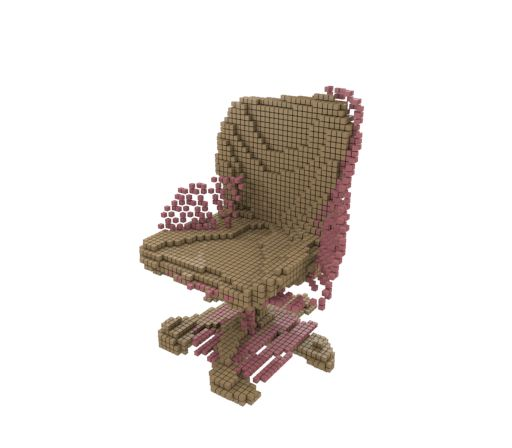
\includegraphics[width=1.5cm,trim={\cropleft cm \croplower cm \cropright cm \cropupper cm},clip]{gexp_clean_chair_high_10_wide_d_vae_aml_3_3_res_396}
	    \end{subfigure}
	    \begin{subfigure}[t]{0.13\textwidth}
	        \vspace{0px}\centering
	        GT\\
	        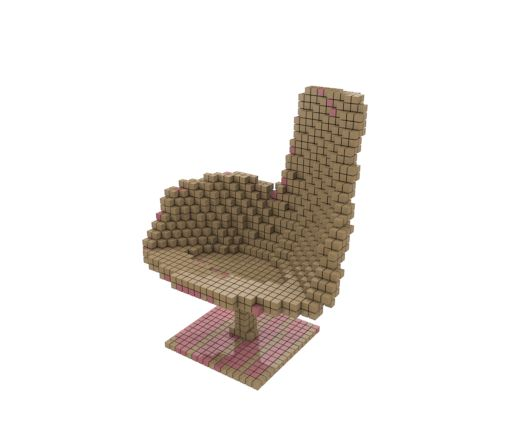
\includegraphics[width=1.5cm,trim={\cropleft cm \croplower cm \cropright cm \cropupper cm},clip]{gdat_modelnet_chair_high_396_bin}
	    \end{subfigure}
	    \begin{subfigure}[t]{0.13\textwidth}
	        \vspace{0px}\centering
	        \AML\\
	        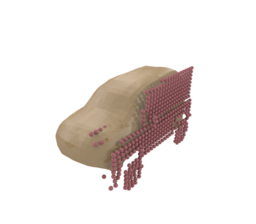
\includegraphics[width=1.5cm,trim={\cropleft cm \croplower cm \cropright cm \cropupper cm},clip]{gexp_clean_low_10_wide_vae_aml_3_2_res_561}
	    \end{subfigure}
	    \begin{subfigure}[t]{0.13\textwidth}
	        \vspace{0px}\centering
	        GT\\
	        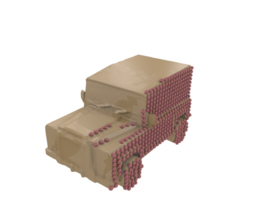
\includegraphics[width=1.5cm,trim={\cropleft cm \croplower cm \cropright cm \cropupper cm},clip]{gdat_shapenet_clean_low_561_gt}
	    \end{subfigure}
	    \begin{subfigure}[t]{0.13\textwidth}
	        \vspace{0px}\centering
	        \AML\\
	        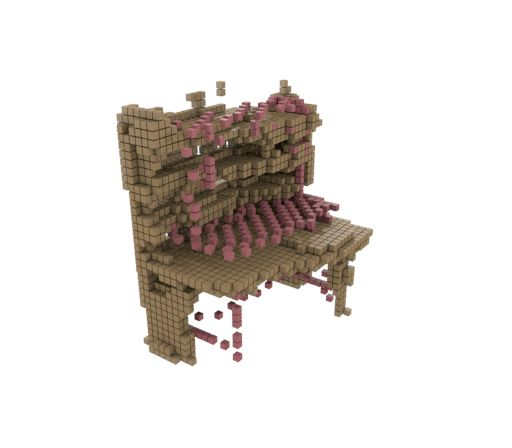
\includegraphics[width=1.5cm,trim={\cropleft cm \croplower cm \cropright cm \cropupper cm},clip]{gexp_clean_desk_medium_10_wide_vae_aml_3_3_res_396}
	    \end{subfigure}
	    \begin{subfigure}[t]{0.13\textwidth}
	        \vspace{0px}\centering
	        \Dai\\
	        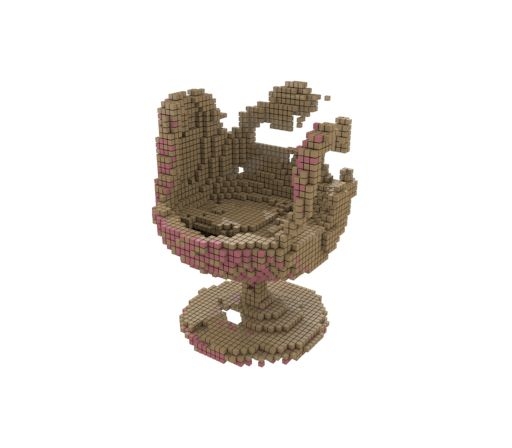
\includegraphics[width=1.5cm,trim={\cropleft cm \croplower cm \cropright cm \cropupper cm},clip]{gexp_clean_chair_high_10_wide_d_sup_3_3_res_528}
	    \end{subfigure}
	    \begin{subfigure}[t]{0.13\textwidth}
	        \vspace{0px}\centering
	        \Dai\\
	        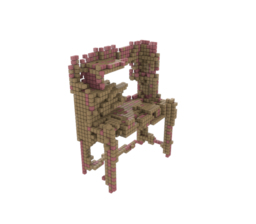
\includegraphics[width=1.5cm,trim={\cropleft cm \croplower cm \cropright cm \cropupper cm},clip]{gexp_clean_desk_medium_10_wide_sup_3_3_res_330}
	    \end{subfigure}
        \subcaption{Difficulties with Exotic Shapes and Fine Structures}
	\end{subfigure}
    \\[4px]
    \begin{subfigure}[t]{0.5\textwidth}
	    \begin{subfigure}[t]{0.15\textwidth}
	        \vspace{0px}\centering
	        \Dai\\
	        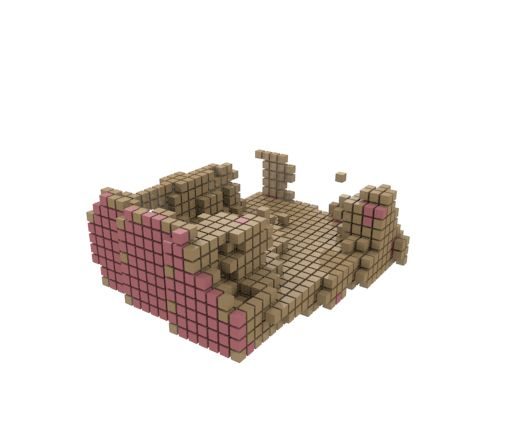
\includegraphics[width=1.5cm,trim={\cropleft cm \croplower cm \cropright cm \cropupper cm},clip]{gexp_clean_modelnet10_low_10_wide_sup_3_3_res_666}
	    \end{subfigure}
	    \begin{subfigure}[t]{0.15\textwidth}
	        \vspace{0px}\centering
	        \AML\\
	        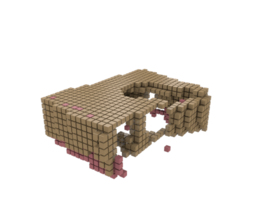
\includegraphics[width=1.5cm,trim={\cropleft cm \croplower cm \cropright cm \cropupper cm},clip]{gexp_clean_modelnet10_low_10_wide_vae_aml_3_3_res_666}
	    \end{subfigure}
	    \begin{subfigure}[t]{0.15\textwidth}
	        \vspace{0px}\centering
	        GT\\
	        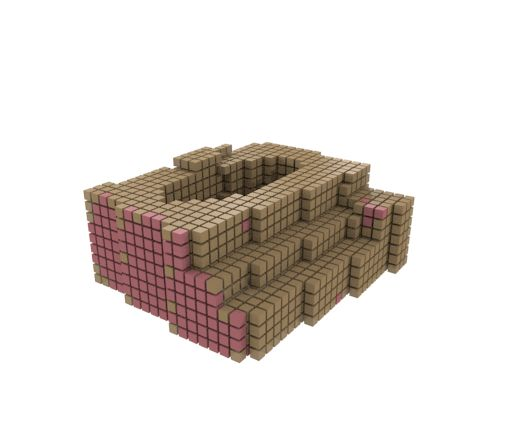
\includegraphics[width=1.5cm,trim={\cropleft cm \croplower cm \cropright cm \cropupper cm},clip]{gdat_modelnet_modelnet10_low_666_bin}
	    \end{subfigure}
	    \begin{subfigure}[t]{0.15\textwidth}
	        \vspace{0px}\centering
	        \Dai\\
	        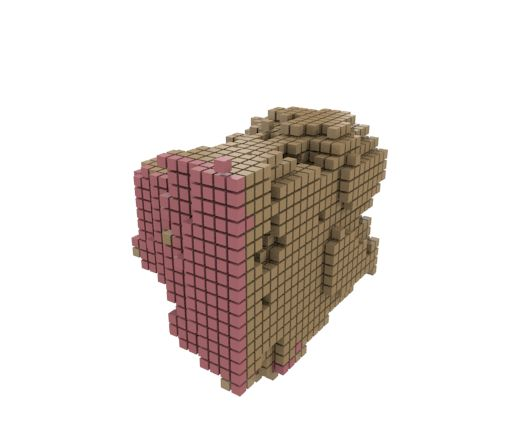
\includegraphics[width=1.5cm,trim={\cropleft cm \croplower cm \cropright cm \cropupper cm},clip]{gexp_clean_modelnet10_low_10_wide_sup_3_3_res_10656}
	    \end{subfigure}
	    \begin{subfigure}[t]{0.15\textwidth}
	        \vspace{0px}\centering
	        \AML\\
	        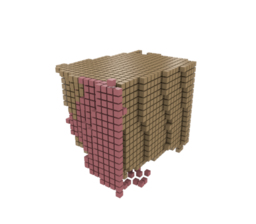
\includegraphics[width=1.5cm,trim={\cropleft cm \croplower cm \cropright cm \cropupper cm},clip]{gexp_clean_modelnet10_low_10_wide_vae_aml_3_3_res_10656}
	    \end{subfigure}
	    \begin{subfigure}[t]{0.15\textwidth}
	        \vspace{0px}\centering
	        GT\\
	        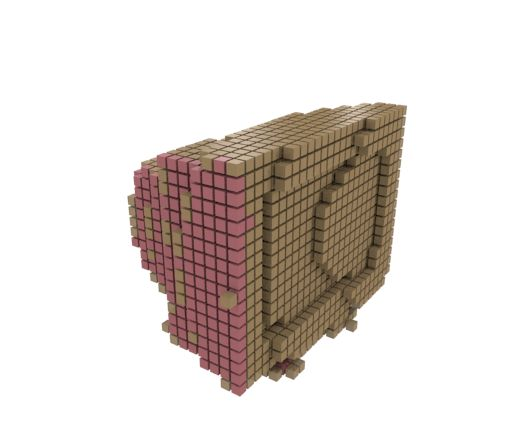
\includegraphics[width=1.5cm,trim={\cropleft cm \croplower cm \cropright cm \cropupper cm},clip]{gdat_modelnet_modelnet10_low_10656_bin}
	    \end{subfigure}
        \subcaption{Difficulties with Multiple Object Categories}
	\end{subfigure}
    }    
    \vspace*{-\figskipcaption px}
    \caption{{\bf Failures Cases.} On the top, we show that \AML has difficulties with exotic shapes, not represented in the latent space; and both \AML and \Dai have difficulties with fine details. The bottom row demonstrates that it is difficult to infer the correct object category from sparse observations, even under full supervision as required by \Dai. Shapes (occupancy grids and mehses) in {\color{rbeige}beige} and observations in {\color{rred}red} from various resolutions.}
    \label{fig:results-failures}
    \vspace*{-\figskipbelow px}
\end{figure}